\documentclass[10pt,twocolumn,letterpaper]{article}

\usepackage{cvpr}
\usepackage{times}
\usepackage{epsfig}
\usepackage{graphicx}
\usepackage{amsmath}
\usepackage{amssymb}

% Include other packages here, before hyperref.

% If you comment hyperref and then uncomment it, you should delete
% egpaper.aux before re-running latex.  (Or just hit 'q' on the first latex
% run, let it finish, and you should be clear).
\usepackage[pagebackref=true,breaklinks=true,letterpaper=true,colorlinks,bookmarks=false]{hyperref}

%%%%%%%%% PAPER ID  - PLEASE UPDATE
\def\cvprPaperID{0446} % *** Enter the CVPR Paper ID here
\def\httilde{\mbox{\tt\raisebox{-.5ex}{\symbol{126}}}}

\begin{document}

%%%%%%%%% TITLE - PLEASE UPDATE
\title{Graph-Based Neural Reconstruction from Skeletonized 3D Networks}  % **** Enter the paper title here

\maketitle
\thispagestyle{empty}


%%%%%%%%% BODY TEXT - ENTER YOUR RESPONSE BELOW

We would like to thank the reviewers for their time.

\section*{Reviewer 1}

\textbf{A1.} 
We thank the reviewer for showing us these four recent papers, and we will cite them in the next revision. 
However, we believe that our work focuses on a slightly different problem. 
Our algorithm corrects the split errors generated by current segmentation algorithms. 
These papers show impressive results but are fundamentally pixel-based methods whereas our method explores higher level error correction. 
We take issue with the statement that ``the paper does not adequately reflect prior art, rendering its own conclusions questionable.'' 
In fact, reviewer 3 wrote ``the list of references is impressive, demonstrating comprehensive knowledge of both recent methods and the application domain.''

\textbf{A2.} 
This claim refers to building on-top of existing segmentation pipelines. 
We will clarify this point in our revision. 
In \textit{Learning to Agglomerate Superpixel Hierarchies}, Jain et al. extract a graph from superpixels generated by a watershed algorithm. 
We, on the other hand, would use the output of \textit{LASH} as input to our framework. 
Then, We extract a graph from this input.

\textbf{A3.} 
We do not agree with the assertion that these are ``drastic'' errors but rather honest mistakes. 
In fact, citing reference [18] for the multicut algorithm is not a mistake at all. 
We use the graph optimization library from Bjoern Andres' website\footnote{http://www.andres.sc/graph.html} which cites [18] (his own work) for the multicut package. 
We will add an additional reference for U-Net that extends the original paper to 3D.
We will update the reference to Funke et al.; this was an accidental LaTex citation omission.

\textbf{B1.} 
We agree that the skeletonization algorithm can improve but our goal for this paper is to use an existing method and explore its application to new ideas.
We chose this method with its corresponding default parameters because it has been used previously for neuron skeletonization.

\textbf{B2.} 
The skeletons from the figures are actually from the anisotropic Kasthuri dataset.

\textbf{B3.} 
We address this in the paper.
The cubic region of interest is actually in nanometers, not voxels.
We further discuss this parameter in the supplemental materials (Sec. 2.1). 
In a future revision we will clarify this better.

From section 4.8, ``Since our CNN only takes as input a region of the label volume we can train on anisotropic data and test on isotropic data.'' 
In the same section we show the results when training on isotropic data (Fig. 9). 

\textbf{B4.} 
We address this in the supplemental material, and will reference it in the future.

\textbf{B5.} 
Without the images, we avoid retraining for every new dataset that has different staining or resolution.
This reduces the amount of expert-labeled ground truth required for every new dataset.
In our experience with our biological collaborators, every dataset has slightly different staining so this offers a large advantage.
We will clarify our thinking.

\textbf{B6.} 
This analysis is provided in Sec. 4.7 and Table 2.

\textbf{B7.} 
We are not using ``lifted'' multicut but only the greedy-edge contraction method.

\textbf{B8. Section 3.4 states that acyclic partitionings are enforced. Since acyclic regions are not an inherent outcome of the multicut algorithm, this requires a modified multicut, but the modification is unspecified.}

\textbf{B9.} 
We reference the possibility for additional constraints using our new novel framework. 
Currently we enforce neurons to be acyclic.
This is a non-trivial constraint for massive datasets where neurons span the entire volume. 
We can later extend our framework 

\textbf{C1.} We use NeuroProof because it scales to terabyte datasets. 
Flood filling networks provide better accuracy but are 25x slower and work on a single neuron at a time. 
For dense reconstruction, NeuroProof is state-of-the-art. 
Variation of Information overcomes previous limitations of Rand error~\cite{lee2017superhuman,nunez2013machine}. 
The SNEMI3D dataset is outdated~\cite{lee2017superhuman}. 

\textbf{C2.} Most of the current state-of-the-art methods are too slow to run on very large datasets, although we will consider other baselines in a future revision.

\section*{Reviewer 2}

Unfortunately the challenge datasets (SNEMI3D, CREMI) are too small for meaningful improvement. The datasets presented in our paper are roughly ten times the size of these challenge datasets. 

\section*{Reviewer 3}

\begin{figure}[h]
	\begin{center}
		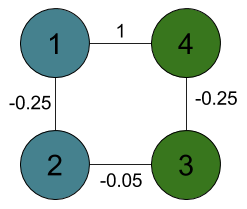
\includegraphics[width=0.32\linewidth]{./figures/MSF.png}
		\caption{Error with minimum spanning forest.}
		\label{figure:msf}
	\end{center}
\end{figure}

\textbf{Address acyclic nature of graph.}

Fig.~\ref{figure:msf} addresses one problem of using a minimum spanning forest where negative edges represent high affinities and positive edges represent low affinities. 
With a multicut formulation, the edge between nodes 1 and 4 will keep the blue and green segments separate.
In a minimum spanning forest nodes 1 and 4 will connect because of the moderate affinity between nodes 2 and 3.

{\small
\bibliographystyle{ieee}
\bibliography{egbib}
}

\end{document}
